\section{System Overview}
Our system consists of four parts: 1) sensing film, 2) capacitance-to-digital converters and 3) automatic mode switching predictor.

\subsection{Sensing Cover}

We built a capacitive sensing grid on a commercially available silicone keyboard cover.
The modified cover was placed over an Apple wireless keyboard.
We connected the ground of the grid to the body of the Apple keyboard to stabilize the readings.
The grid consists of 58 vertical and 20 horizontal 30 AWG copper wires.
With mutual capacitance sensing techniques, each cross point of vertical and horizontal wires can be a single sensing point, so the film can capture a 58x20 frame.
The sensing resolution could be higher if the conductive pattern would be printed directly on the cover with higher line density.
With this modified keyboard cover, we can enable touch sensing capability on any keyboard by simply putting it over an unmodified keyboard.

\subsection{Capacitance To Digital Converters(CDC)}

% To measure the change of mutual capacitance value of the sensor grid cross points, we referenced the design of SmartSkin \cite{smartskin} and built a customized CDC.
We adopted the CDC design of SmartSkin \cite{smartskin} to measure the change of mutual capacitances at the sensor grid intersections. Here we briefly highlight our changes cover \cite{smartskin}. 
The main idea of this design is to measure the signal reduction of the square wave signal passed through the sensor film, which can be viewed as a very small capacitor.
The square wave signal generated by a programmable clock generator is passed into sensor films through analog demultiplexers, so we can raster scan through all the 58 vertical wires by switching between the channels.
20 OP-Amps are connected to the horizontal wires of the sensor grid, amplifying the weakened signal by a factor of 5 for further processing.
% We remove the noise generated by circuits nearby with a simple lock-in amplifier, the lock-in amplifier takes noisy signals as input and outputs the signal strength of the target frequency.
The CDC also has an analog subtractor for hardware-based background substraction.
% The CDC samples the output level of the analog subtractor with a 10-bit Analog to Digital Converter(ADC) and sends the data back to a computer via a standard USB serial device.
% Although our system is quite large, the whole capacitive sensing system can be designed to be much smaller and portable when produced commercially, since the technique used is in essence the same as the capacitive technology in smart phones.
The CDC currently is capable of raster scanning through the sensor grid at 13 Hz.
% The CDC subtracts the background image internally.
Calibration of the sensor is done by sampling through the sensor grid for 10 times.
The data generated by the CDC can form a 58x20 pixels resolution. Each pixel has 10-bit intensity value ranging from 0 to 1023.
The sensor grid only responds to conductive objects in a very short range($<$0.2cm).

\begin{figure}[!h]
\centering
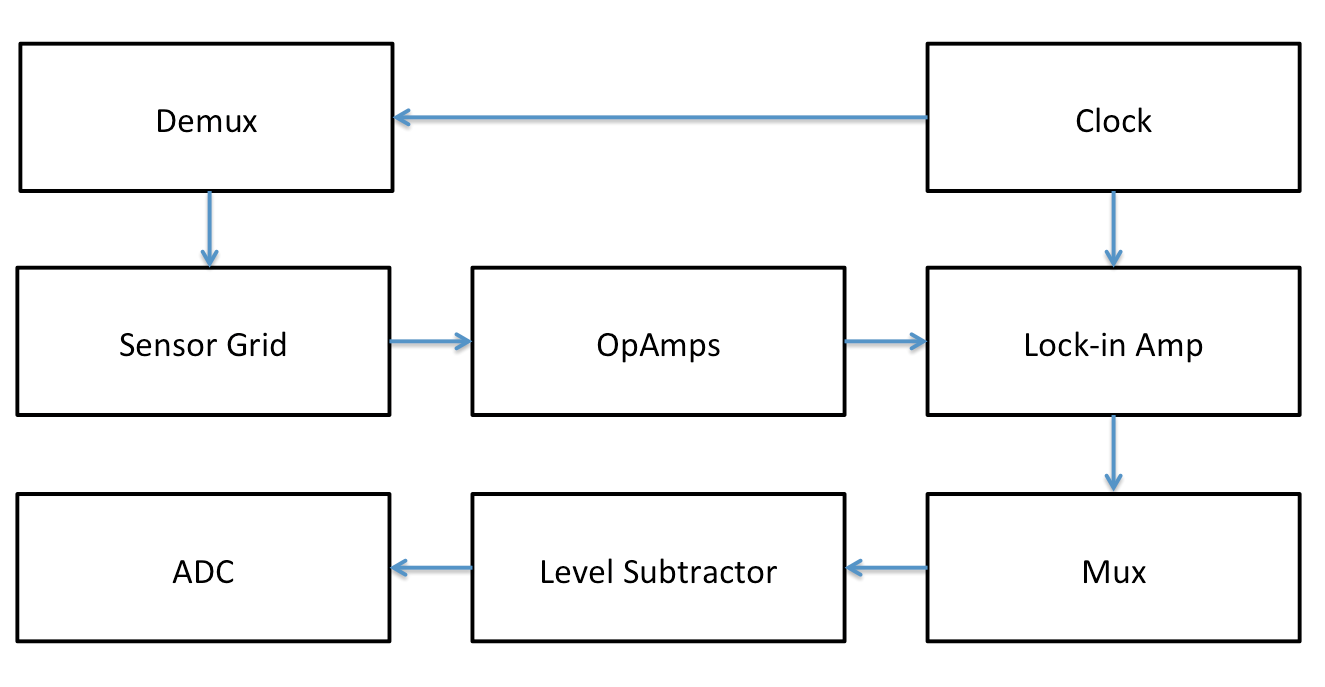
\includegraphics[width=0.8\columnwidth]{figures/figure2.png}
\caption{CDC circuit diagram. The switch and RC low-pass filter are the main components of the lock-in amplifier.}
\label{fig:figure2}
\end{figure}

% 01/09: 可移除這個subsection title,內文緊接前面小節。
% \subsection{Sensor Characteristics and Data}

% The CDC currently is capable of raster scanning through the sensor grid at 13 Hz.
% The CDC subtracts the background image internally.
% Calibration of the sensor is done by sampling through the sensor grid for 10 times.
% The data generated by the CDC can form a 58x20 pixels resolution, each pixel has 10-bit intensity value ranging from 0 to 1023.
% The sensor grid only responds to conductive objects in a very short range($<$0.2cm).


\subsection{Signal Processing}

The 58x20 10-bit intensity image is scaled up to 464x160 10-bit image with nearest-neighbor interpolation to provide a more accurate cursor positioning capability. (Figure~\ref{fig:figure1}.D)
A Gaussian filter is then applied to the image for smoother blob images.
Each row of the filtered image is subtracted with the mean of the row since we found that the sensor value will be interfered when there are some other touch points on the same horizontal sensing wire.(Figure~\ref{fig:figure1}.E)
The image is binarized with a simple local adaptive thresholding algorithm.
Finally, the system detects blobs in the binarized image as touched points. (Figure~\ref{fig:figure1}.F)
Calculated blob positions are filtered with a Kalman filter to stabilize blob position and make cursor controlling possible.

% \subsection{Automatic Mode Switching Prediction}

% We also implemented Motion Signature \cite{96bytes} to recognize whether the user is trying to use the pointing device or not.
% % Since the sample rate is relatively lower (13Hz) compared to the original condition(325Hz), we reduced the referenced frames to only 30 frames in the process of building motion history images(MHI).
% Since our sensor's sampling rate of 13Hz is much lowaer than the sensor used in \cite{96bytes}(325Hz), we only used 30 frames of raw signal to build MHIs. 
% Also, we removed binary-MHI(bMHI) from the original MHI implementation because intensity-MHI already provides enough accuracy for recognizing user intention.
% We classify the calculated MHIs with Random Decision Forests(RDF), the same classifier used in Type–Hover–Swipe \cite{96bytes}.
% %reviewer 9th request
% With our hardware system, we can extract touch areas from the image collected with the capacitive sensor grid. Therefore, our system can recognize where the moving touch point is even if the second hand rests on the keyboard. 